\documentclass[11pt]{article}

\usepackage[a4paper,margin=27mm]{geometry}
\usepackage[T1]{fontenc}
\usepackage[utf8]{inputenc}
\usepackage{lmodern}
\usepackage{microtype}
\usepackage{amsmath,amssymb}
\usepackage{array,booktabs,longtable}
\usepackage{graphicx}
\usepackage{float}
\usepackage{xcolor}
\usepackage{tikz}
\usetikzlibrary{arrows.meta}
\usepackage[
  colorlinks=true,
  linkcolor=blue!65!black,
  urlcolor=blue!65!black,
  citecolor=blue!65!black
]{hyperref}

\definecolor{linkblue}{RGB}{20,70,190}
\definecolor{paperfill}{RGB}{236,253,245}
\definecolor{paperline}{RGB}{22,163,74}
\definecolor{boundaryfill}{RGB}{238,242,255}
\definecolor{boundaryline}{RGB}{79,70,229}

\newcommand{\decl}[1]{\nolinkurl{#1}}
\newcommand{\mstmt}[2]{#1~\textcolor{linkblue}{#2}}

\setlength{\parindent}{1.35em}
\setlength{\parskip}{0pt}
\setlength{\tabcolsep}{3.5pt}
\renewcommand{\arraystretch}{1.08}
\setlength{\LTcapwidth}{\textwidth}

\begin{document}

\appendix
\section{Lean correspondence}
\label{app:lean-correspondence}

The accompanying Lean development follows the proof architecture of
Sections~4 and~5 of
\href{https://arxiv.org/abs/2601.23213}{the conditional-entropy manuscript}.
Figure~\ref{fig:lean-dependencies} gives the dependency graph, with arrows
pointing from a manuscript conclusion to its checked ingredients. Green boxes
are paper-facing coefficient cores and blue boxes are standalone bridge or
boundary proofs. Table~\ref{tab:lean-correspondence} records the
statement-by-statement correspondence.

The parenthetical value in each box is the number of Lean declarations
introduced with \decl{theorem} or \decl{lemma}. The counts are disjoint and
sum to 36. Every one of these declarations is checked with Lean~4.32.2 and
Mathlib~4.32.2. The source contains no \decl{sorry}, \decl{admit}, or
project-specific \decl{axiom}; a separate kernel audit prints the axiom
dependencies of the public declarations.

The word ``core'' is deliberate. The present development verifies the finite
coefficient and order-theoretic consequences of the manuscript. The
general-measure discretisation, differentiated R\'enyi integral, and
high-dimensional localisation limits remain explicit analytic boundaries.
They are neither asserted as Lean theorems nor hidden behind additional
axioms. The source is available at
\href{https://github.com/robertorubboli/conditional-entropy-characterisation}
{github.com/robertorubboli/conditional-entropy-characterisation}.

\renewcommand{\thefigure}{\thesection.\arabic{figure}}
\setcounter{figure}{0}

\begin{figure}[H]
  \centering
  \resizebox{\textwidth}{!}{%
  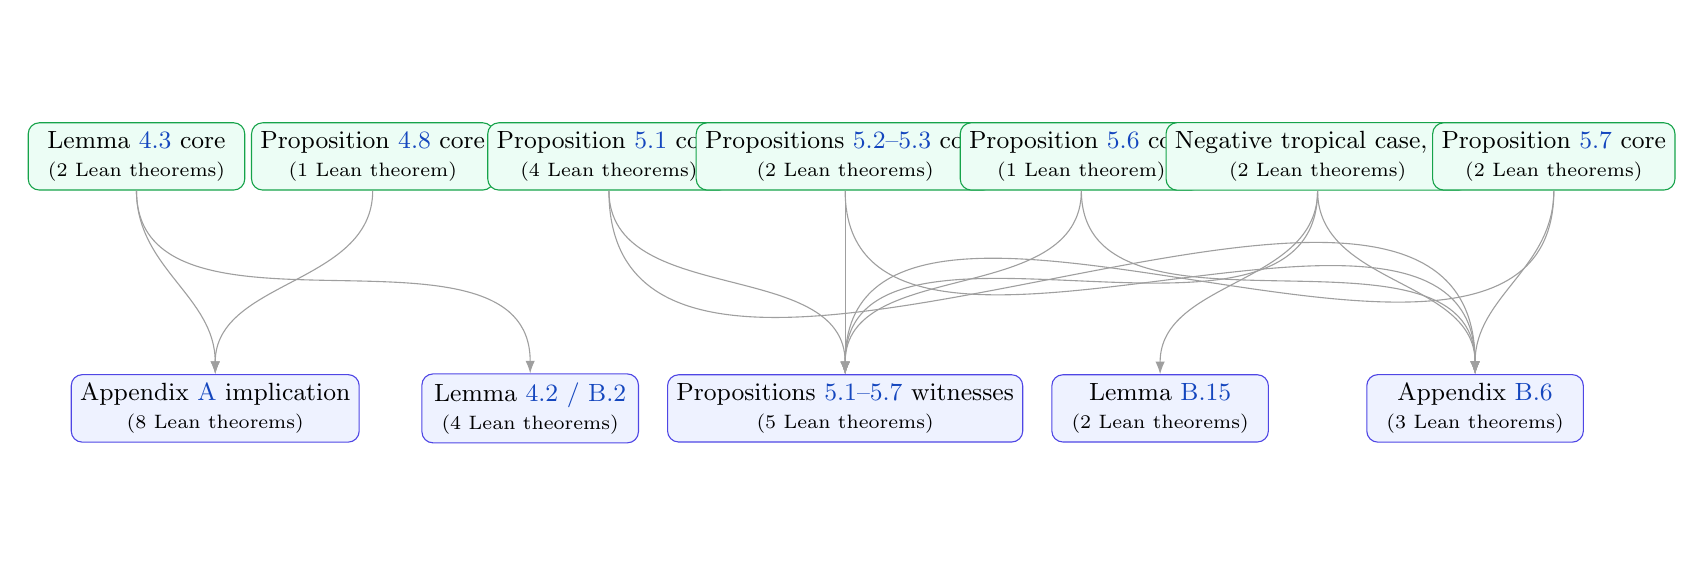
\begin{tikzpicture}[
      x=1cm,y=1cm,
      box/.style={draw,rounded corners,align=center,inner sep=3.2pt,
                  font=\small,minimum width=2.75cm},
      paper/.style={box,fill=paperfill,draw=paperline},
      boundary/.style={box,fill=boundaryfill,draw=boundaryline},
      every edge/.style={draw,gray!75,-{Latex[length=1.6mm]}}]

    \node[paper] (l43) at (-9,3.2)
      {Lemma \textcolor{linkblue}{4.3} core\\[-1pt]\scriptsize(2 Lean theorems)};
    \node[paper] (p48) at (-6,3.2)
      {Proposition \textcolor{linkblue}{4.8} core\\[-1pt]\scriptsize(1 Lean theorem)};
    \node[paper] (p51) at (-3,3.2)
      {Proposition \textcolor{linkblue}{5.1} core\\[-1pt]\scriptsize(4 Lean theorems)};
    \node[paper] (p523) at (0,3.2)
      {Propositions \textcolor{linkblue}{5.2--5.3} core\\[-1pt]\scriptsize(2 Lean theorems)};
    \node[paper] (p56) at (3,3.2)
      {Proposition \textcolor{linkblue}{5.6} core\\[-1pt]\scriptsize(1 Lean theorem)};
    \node[paper] (nt) at (6,3.2)
      {Negative tropical case, \S\textcolor{linkblue}{5}\\[-1pt]\scriptsize(2 Lean theorems)};
    \node[paper] (p57) at (9,3.2)
      {Proposition \textcolor{linkblue}{5.7} core\\[-1pt]\scriptsize(2 Lean theorems)};

    \node[boundary] (appa) at (-8,0)
      {Appendix \textcolor{linkblue}{A} implication\\[-1pt]\scriptsize(8 Lean theorems)};
    \node[boundary] (b2) at (-4,0)
      {Lemma \textcolor{linkblue}{4.2 / B.2}\\[-1pt]\scriptsize(4 Lean theorems)};
    \node[boundary] (witness) at (0,0)
      {Propositions \textcolor{linkblue}{5.1--5.7} witnesses\\[-1pt]\scriptsize(5 Lean theorems)};
    \node[boundary] (b15) at (4,0)
      {Lemma \textcolor{linkblue}{B.15}\\[-1pt]\scriptsize(2 Lean theorems)};
    \node[boundary] (b6) at (8,0)
      {Appendix \textcolor{linkblue}{B.6}\\[-1pt]\scriptsize(3 Lean theorems)};

    \draw (l43) edge[out=-90,in=90] (appa);
    \draw (l43) edge[out=-90,in=90] (b2);
    \draw (p48) edge[out=-90,in=90] (appa);
    \draw (p51) edge[out=-90,in=90] (witness);
    \draw (p51) edge[out=-90,in=90] (b6);
    \draw (p523) edge[out=-90,in=90] (witness);
    \draw (p523) edge[out=-90,in=90] (b6);
    \draw (p56) edge[out=-90,in=90] (witness);
    \draw (p56) edge[out=-90,in=90] (b6);
    \draw (nt) edge[out=-90,in=90] (witness);
    \draw (nt) edge[out=-90,in=90] (b15);
    \draw (nt) edge[out=-90,in=90] (b6);
    \draw (p57) edge[out=-90,in=90] (witness);
    \draw (p57) edge[out=-90,in=90] (b6);
  \end{tikzpicture}%
  }
  \caption{Dependency graph for the checked Lean core. Parenthetical counts
  total 36 theorem/lemma declarations.}
  \label{fig:lean-dependencies}
\end{figure}

% Starting at one makes this Table A.2, following Figure A.1 as in the
% reference appendix.
\renewcommand{\thetable}{\thesection.\arabic{table}}
\setcounter{table}{1}

\begingroup
\small
\begin{longtable}{@{}%
  >{\raggedright\arraybackslash}p{0.235\textwidth}%
  >{\raggedright\arraybackslash}p{0.49\textwidth}%
  >{\centering\arraybackslash}p{0.07\textwidth}%
  >{\raggedright\arraybackslash}p{0.14\textwidth}@{}}
\caption{Correspondence between manuscript statements and Lean declarations.
The counts are disjoint.}\label{tab:lean-correspondence}\\
\toprule
Manuscript statement & Lean declaration & Count & Status\\
\midrule
\endfirsthead
\multicolumn{4}{c}{\tablename\ \thetable\ continued}\\
\toprule
Manuscript statement & Lean declaration & Count & Status\\
\midrule
\endhead
\midrule
\multicolumn{4}{r}{Continued on the next page}\\
\endfoot
\bottomrule
\endlastfoot

Appendix A, conditioning implication &
\decl{isSuperadditive_of_concave_posHomogeneous};
\decl{isSubadditive_of_convex_posHomogeneous};
\decl{superadditive_finset_sum};
\decl{subadditive_finset_sum};
\decl{columnLift_pushConditioning_ge};
\decl{columnLift_pushConditioning_le};
\decl{conditioning_monotone_of_concave};
\decl{conditioning_antitone_of_convex}
& 8 & Formalized\\[2pt]

\mstmt{Lemma}{4.2} / \mstmt{Lemma}{B.2}, monomial curvature &
\decl{monomialCurvature_eq_neg_variance};
\decl{monomialCurvature_nonpos_of_nonneg};
\decl{coefficient_mem_Icc_of_curvature_nonpos};
\decl{monomialCurvature_pos_of_negative_coefficient}
& 4 & Formalized core\\[2pt]

\mstmt{Propositions}{5.1--5.7}, scalar witnesses &
\decl{two_positive_stationary_witness};
\decl{negative_tail_concavity_obstruction};
\decl{excessive_lower_moment_concavity_obstruction};
\decl{shannon_atom_concavity_obstruction};
\decl{positive_tail_derivation_obstruction}
& 5 & Formalized core\\[2pt]

\mstmt{Lemma}{4.3}, finite coefficient signs &
\decl{positiveTemperate_coefficients_nonnegative};
\decl{negativeTemperate_two_coefficient_curvature}
& 2 & Formalized core\\[2pt]

\mstmt{Proposition}{4.8}, coefficient consequence &
\decl{derivation_supported_below_has_no_upper_obstruction}
& 1 & Formalized core\\[2pt]

\mstmt{Proposition}{5.1}, coefficient conclusions &
\decl{positiveTemperate_shannon_atom_zero};
\decl{positiveTemperate_no_upper_moment};
\decl{positiveTemperate_lowerMoment_le_one};
\decl{positiveTemperate_necessary}
& 4 & Formalized core\\[2pt]

\mstmt{Propositions}{5.2--5.3}, exceptional moment &
\decl{negativeTemperate_truncated_moment};
\decl{negativeTemperate_exceptional_moment}
& 2 & Formalized core\\[2pt]

\mstmt{Proposition}{5.6}, two-upper-cell contradiction &
\decl{negativeTemperate_atMostOneUpperCell}
& 1 & Formalized core\\[2pt]

Negative tropical necessity in Section~5 &
\decl{negativeTropical_moment_nonnegative};
\decl{negativeTropical_exceptional_moment}
& 2 & Formalized core\\[2pt]

\mstmt{Proposition}{5.7}, derivation necessity &
\decl{derivation_no_positive_upper_tail};
\decl{derivation_necessary}
& 2 & Formalized core\\[2pt]

\mstmt{Lemma}{B.15}, exact stationarity &
\decl{stationarityCorrection_dot};
\decl{stationarityCorrection_tendsto}
& 2 & Formalized\\[2pt]

Appendix B.6, finite midpoint contradictions &
\decl{not_concave_of_strict_midpoint_valley};
\decl{not_convex_of_strict_midpoint_peak};
\decl{not_quasiConvex_of_strict_midpoint_peak}
& 3 & Formalized\\[2pt]

\midrule
\mstmt{Proposition}{4.4} and analytic Lemmas B.1, B.3--B.13 &
General-measure approximation, differentiation, and localisation
& 0 & Analytic boundary\\

\midrule
\multicolumn{2}{r}{\textbf{Checked theorem/lemma declarations}}
& \textbf{36} & \\

\end{longtable}
\endgroup

\end{document}
